% Written By Enoch Yu
% Downloaded from archive.enochyu.com

\documentclass{article}

\usepackage{amsmath}
\usepackage{amssymb}
\usepackage{amsthm}
\usepackage{mathtools}

\usepackage[margin=1in, headsep=15pt]{geometry}
\usepackage{lastpage}
\usepackage{fancyhdr}
\fancyhead[R]{Enoch Yu}
\fancyfoot[C]{Page \thepage \hspace{1pt} of \pageref{LastPage}}
\pagestyle{fancy}
\usepackage{parskip}

\usepackage{enumitem}
\usepackage[dvipsnames]{xcolor}
\usepackage[normalem]{ulem}
\usepackage{url}
\usepackage{hyperref}
\hypersetup{
    colorlinks=true,
    linkcolor=black,
    filecolor=magenta,      
    urlcolor=cyan,
    pdftitle={7.15.2025 AMC 10 Free Class Preview Homework Solution},
    pdfpagemode=FullScreen,
}
\usepackage{tabularx}
\usepackage{arydshln}
\usepackage{float}
\usepackage{pdfpages}

\usepackage{tikz}
\usetikzlibrary{calc, angles, shapes.geometric}
\usepackage{tkz-euclide}
\usepackage{pgfplots}
\pgfplotsset{compat=1.9}
\usepackage[font=small,labelfont=bf]{caption}

\newtheorem{theorem}{Theorem}[section]
\newtheorem{lemma}[theorem]{Lemma}
\newtheorem*{lemma*}{Lemma}
\newtheorem{sublemma}{Lemma}[section]
\newtheorem{proposition}{Proposition}
\newtheorem{corollary}{Corollary}[theorem]
\newtheorem{example}{Example}[section]
\newtheorem*{example*}{Example}
\newenvironment{solution}{\begin{trivlist}\item[]{\bf Solution}}{\qed \end{trivlist}}

\title{7.15.2025 AMC 10 Free Class Preview Homework Solution}
\author{Enoch Yu}
\date{July 2025}

\begin{document}

\maketitle

\subsection*{Problem}
If the roots of the equation $2kx^2 - (3k + 2)x + 2k - 1
= 0$ differ by 1, find the positive value of $k$.

\begin{solution}
Let $\alpha$ and $\beta$ be the roots of the equation.
Therefore, $\alpha + \beta = \frac{3k - 2}{2k}$ and
$\alpha\beta = \frac{2k - 1}{2k}$. Moreover, the following
equations are true.
\begin{align*}
    \left( \frac{3k - 2}{2k} \right)^2
        - 4 \left( \frac{2k - 1}{2k} \right) &= 1 \\
    \frac{9k^2 - 12k + 4}{4k^2} - \frac{4k - 2}{k} &= 1 \\
    9k^2 - 12k + 4 - 16k^2 + 8k &= 4k^2 \\
    11k^2 - 20k - 4 &= 0 \\
    (11k + 2)(k - 2) &= 0 \\
    \therefore k &= \boxed{2}
\end{align*}
\end{solution}

\subsection*{Problem}
Solve the system of equations.
\[
\begin{cases}
    x + xy + y &= 11 \\
    x^2y + xy^2 &= 30
\end{cases}
\]
\begin{solution}
Let $a = x + y$ and $b = xy$. Therefore, $a + b = 11$
and $ab = 30$. Let $a$ and $b$ be the roots of the
following equation.
\[
t^2 - 11t + 30 = 0
\]
Therefore, $a = 5$ and $b = 6$, or $a = 6$ and $b = 5$.
From the first case, the pairs of $(x, y)$ are $(2, 3)$
and $(3, 2)$. From the second case, the pairs of $(x, y)$
are $(1, 5)$ and $(5, 1)$. Therefore, the roots of the
system of equations are $\boxed{(2, 3), (3, 2), (1, 5), (5, 1)}$.
\end{solution}

\section*{\textcolor{BrickRed}{Hard Problems}}
\subsection*{Problem}
A Circle $O$ of radius $r$ is inscribed to $\triangle{ABC}$
at $D$, $E$, and $F$. $\angle{C} = 60^\circ$. The length
of the side opposite to $\angle{C}$ is $c = \sqrt{3}$.
Find the range of $r$.
\begin{solution}
\begin{center}
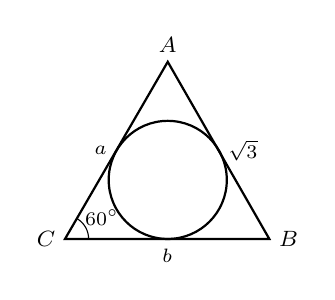
\begin{tikzpicture}[scale=1.5]
    \coordinate (A) at (0.87, 1.5);
    \coordinate (B) at (1.73, 0);
    \coordinate (C) at (0, 0);
    \coordinate (O) at (0.87, 0.5);

    \draw[thick] (A) -- (B) -- (C) -- cycle;
    \draw[thick] (O) circle (0.5);

    \node[above] at (A) {\footnotesize $A$};
    \node[right] at (B) {\footnotesize $B$};
    \node[left] at (C) {\footnotesize $C$};

    \node[left] at ($(A)!0.5!(C)$) {\scriptsize $a$};
    \node[right] at ($(A)!0.5!(B)$) {\scriptsize $\sqrt{3}$};
    \node[below] at ($(B)!0.5!(C)$) {\scriptsize $b$};

    \draw pic["\scriptsize $60^\circ$", draw=black, angle radius=0.3cm, angle eccentricity=1.8] {angle=B--C--A};
\end{tikzpicture}
\end{center}
From the diagram, notice that the values of $a + b$
and $ab$ could be written in terms of $r$.
\begin{align*}
    a - \tan60^\circ \cdot r + b - \tan60^\circ \cdot r
    &= \sqrt{3} \\
    a + b
    &= \sqrt{3}(2r + 1) \\
    \frac{r(a + b + \sqrt{3})}{2}
    &= \frac{\sqrt{3}ab}{4} \\
    \frac{r\left( \sqrt{3}(2r + 1) + \sqrt{3} \right)}{2}
    &= \frac{\sqrt{3}ab}{4} \\
    ab &= 2r(2r + 2)
\end{align*}
Let $a$ and $b$ be the root of the equation
\[
t^2 - \sqrt{3}(2r + 1) + 4r^2 + 4r = 0
\]
Discriminant could be used since $a$ and $b$
are positive numbers.
\begin{align*}
    12r^2 + 12r + 3 - 16r^2 - 16r &\geq 0 \\
    4r^2 + 4r - 3 &\leq 0 \\
    (2r + 3)(2r - 1) &\leq 0 \\
    \therefore \boxed{0 < r \leq \frac{1}{2}}
\end{align*}
\end{solution}

\subsection*{Problem}
Show that there is one and only one of real numbers
$x$, $y$, and $z$ that is at least $\sqrt[3]{4}$ if
$x + y + z = 0$ and $xyz = 1$.
\begin{proof}
WLOG, let $x \leq y < z$ and let $x$ and $y$ be the
solution to the following equation.
\[
t^2 + zt + \frac{1}{z} = 0
\]
Using discriminant, $z^2 - \frac{4}{z} \geq 0$.
Because $z$ must be a positive number, $z^3 \geq 4$.
In other words, only $z \geq \sqrt[3]{4}$.
\end{proof}

\subsection*{Problem}
Solve for real $x$, $y$, and $z$.
\[
\begin{cases}
    x + y &= 2 \\
    xy - z^2 &= 1
\end{cases}
\]
\begin{solution}
Notice let $x$ and $y$ be the solution to the
following equation.
\[
t^2 - 2t + 1 + z^2 = 0
\]
Using discriminant, it is evident that $z = 0$ and
$z = y = 1$. Thus, the solution is $\boxed{(1, 1, 0)}$.
\end{solution}
\end{document}

